% !TEX root = ../manuscript.tex

\chapter{Dynamical Systems on Lie Groups}

Having defined derivatives on Lie Groups we can introduce dynamical systems that evolve on Lie Groups. ODEs can be defined in multiple ways depending on how derivatives are handled. Consider a system $\X(t)$ whose state can be interpreted as a mapping $\mathbb{E}(1) \rightarrow \cM$.

If $^\X \a$ is the body derivative the system can be written with an equation involving the right derivative:
\begin{equation}
  \mathrm{d}^r \X_t = {^\X}\a(t), \quad {^\X}\a(t) \in T_\X \cM.
\end{equation}
The same system can be written in terms of the derivative ${^\id}\a(t)$ in the global tangent frame $T_\id \cM$ using the left derivative:
\begin{equation}
  \mathrm{d}^l \X_t = {^\id}\a(t), \quad {^\id}\a(t) \in T_\id \cM.
\end{equation}
We can also write the global derivative as
\begin{equation}
  \mathrm{D} \X_t = \X \circ {^\X}{\hat\a}(t) = {^\id}{\hat\a}(t) \circ \X,
\end{equation}
where the derivative is with respect to the coefficients of the matrix $\X$. Naturally, as long as
\begin{equation}
  \label{eq:velocity_at_identity}
  {^\id \a(t)} = \bAd_{\X(t)} {^\X \a}(t)
\end{equation}
all these formulations describe the same dynamical system, which can be readily seen from \eqref{eq:derivative_trans}.

\section{Dynamical systems and the exponential map}

Consider the dynamical system $\X(t) = x_0 \circ \exp(t \a)$, evaluating the right derivative with respect to $t$ gives
\begin{equation}
  \mathrm{d}^r \X_t = \lim_{\tau \rightarrow 0} \frac{\exp(t \a)^{-1} \circ \exp((t + \tau) \a)}{\tau} = \lim_{\tau \rightarrow 0} \frac{\exp(\tau \a)}{\tau} = \a.
\end{equation}
It follows that $\X_0 \circ \exp (t \a)$ is the solution to the ordinary differential equation
\begin{equation}
  \begin{cases}
    \mathrm{d}^r \X_t = \a, \\
    \X(0) = \X_0.
  \end{cases}
\end{equation}


\todo[inline]{Show connection with formulas that map velocities in a rotating frame}

\subsection{Geometric Numerical Integration}

\todo[inline]{Geometric RK scheme}



\section{A Stabilizing Lie Group Controller}

Consider the system
\begin{equation}
  \begin{aligned}
    \mathrm{d}^r \X_t & = v \\
    \mathrm{d}^r v_t & = u
  \end{aligned}
\end{equation}
where $u$ is a control input, and the objective of tracking a twice differentiable trajectory $\X_d(t)$ with first and second right-derivatives $v_d$ and $a_d$. Consider the error
\begin{equation}
  e_\X \coloneq \X_d \ominus_r \X,
\end{equation}
with derivative
\begin{equation}
  \mathrm{d}^r (e_\X)_t \overset{\eqref{eq:d_rminus_fst},\eqref{eq:d_rminus_snd}}= \left(\mathrm{d}^r \exp_{e_\X} \right)^{-1} \mathrm{d}^r \X_d - \left(\mathrm{d}^l \exp_{e_\X} \right)^{-1} \mathrm{d}^r \X = \left(\mathrm{d}^l \exp_{e_\X} \right)^{-1} (\bAd_{\exp(e_\X)} v_d - v).
\end{equation}
Note that $\bAd_{\exp(e_\X)} = \exp \ad_{e} = \sum_{k \geq 0} \frac{\ad_e}{k!}$ can typically be found on closed form via the usual expansion tricks. Let $e_v \coloneq \bAd_{\exp(e_\X)} v_d - v$ be the velocity error in the body frame; we then have the double intergrator-like error system
\begin{equation}
  \begin{aligned}
    \frac{\mathrm{d}}{\mathrm{d}t} e_\X &= \left(\mathrm{d}^l \exp_{e_\X} \right)^{-1} e_v,\\
    \frac{\mathrm{d}}{\mathrm{d}t} e_v &= \frac{\mathrm{d}}{\mathrm{d}t} \left( \bAd_{\exp(e_\X)} v_d\right) - u,
  \end{aligned}
\end{equation}
Where we can further simplify
\begin{equation}
  \frac{\mathrm{d}}{\mathrm{d}t} \left( \bAd_{\exp(e_\X)} v_d\right) \overset{\eqref{eq:bAd_dl}}= \left[ \mathrm{d}^l \exp_{e_\X} \dot e_\X,  \bAd_{\exp(e_\X)} v_d \right] + \bAd_{\exp(e_\X)} \dot v_d = \left[ e_v,  \bAd_{\exp(e_\X)} v_d \right] + \bAd_{\exp(e_\X)} \dot v_d.
\end{equation}
If we further consider an input on the form $u = \left[ e_v,  \bAd_{\exp(e_\X)} v_d \right] + \bAd_{\exp(e_\X)} \dot v_d + k_p \textcolor{red}{\left( \mathrm{d}^l \exp_{e_\X} \right)^{-T}} e_\X + k_d e_v$ that cancels out the contribution from $v_d$ and adds PD feedback terms the closed-loop dynamics become
\begin{equation}
  \begin{aligned}
    \frac{\mathrm{d}}{\mathrm{d}t} e_\X &= \left(\mathrm{d}^l \exp_{e_\X} \right)^{-1} e_v,\\
    \frac{\mathrm{d}}{\mathrm{d}t} e_v &= -k_p \textcolor{red}{\left( \mathrm{d}^l \exp_{e_\X} \right)^{-T}} e_\X - k_d e_v.
  \end{aligned}
\end{equation}
Now consider a Lyapunov candidate function on the form
\begin{equation}
  V = \frac{k_p}{2} \| e_\X \|^2 + \frac{1}{2} \| e_v \|^2 + c \left \langle e_v, e_\X \right \rangle \geq \frac{1}{2} \begin{bmatrix} \| e_\X \| \\ \| e_v \| \end{bmatrix}^T \begin{bmatrix} k_p & -c \\ -c & 1 \end{bmatrix} \begin{bmatrix} \| e_\X \| \\ \| e_v \| \end{bmatrix},
\end{equation}
where $c$ is s.t. $k_p - c^2 \geq 0$ so that the matrix is positive definite. Its derivative evaluates to
\begin{equation*}
  \begin{aligned}
    \dot V &= k_p \left \langle e_\X, \left( \mathrm{d}^l \exp_{e_\X} \right)^{-1} e_v \right \rangle - k_p \left \langle e_v,  \textcolor{red}{\left( \mathrm{d}^l \exp_{e_\X} \right)^{-T}} e_\X \right \rangle - k_d \| e_v \|^2 + c \left \langle \dot e_v, e_\X \right \rangle + c \left \langle e_v, \dot e_\X \right \rangle \\
    & = - k_d \| e_v \|^2 - c \left \langle k_p \textcolor{red}{\left( \mathrm{d}^l \exp_{e_\X} \right)^{-T}} e_\X + k_d e_v, e_\X \right \rangle + c \left \langle e_v, \left(\mathrm{d}^l \exp_{e_\X} \right)^{-1} e_v \right \rangle \\
    & = -k_d \| e_v \|^2 - c k_p \| e_\X \|^2 - c k_d \left \langle e_v, e_\X \right \rangle + c \left \langle e_v, \left(\mathrm{d}^l \exp_{e_\X} \right)^{-1} e_v \right \rangle - c k_p \left \langle ( \textcolor{red}{(\mathrm{d}^l \exp_{e_\X})^{-T}} - I) e_\X , e_\X \right \rangle \\
    & \leq -k_d \| e_v \|^2 - c k_p \| e_\X \|^2 + c k_d \| e_v \| \| e_\X \| + c \lambda_{\textrm{max}}\left( \left( \mathrm{d}^l \exp_{e_\X} \right)^{-1} \right) \| e_v \|^2 + c k_p \lambda_{\textrm{max}} \left( \textcolor{red}{\left(\mathrm{d}^l \exp_{e_\X} \right)^{-1}} - I \right) \| e_\X \|^2.
  \end{aligned}
\end{equation*}

\begin{itemize}
  \item Eigenvalues of $(\mathrm{d}^l \exp_{e_\X})^{-1}$ can be shown to be on the form $\frac{\lambda}{e^{\lambda} - 1} = \sum_{k=0}^\infty \frac{B_n}{n!} \lambda^n$, where $\lambda$ is an eigenvalue of $\ad_e$.
  \item Zero is always an eigenvalue of $\ad_e$ since $\ad_e e = 0$ due to it being a commutator (the corresponding eigenvalue of $(\mathrm{d}^l \exp_e)^{-1}$ is 1
  \item Often, the eigenvalues of $\ad_e$ are purely imaginary. The corresponding eigenvalues of $(\mathrm{d}^l \exp_{e_\X})^{-1}$ are
  \begin{equation}
    \frac{i \lambda}{e^{i \lambda} - 1} = \frac{i \lambda e^{-i \lambda / 2}}{e^{i \lambda / 2} - e^{- i \lambda / 2}} = \frac{i \lambda e^{-i \lambda / 2}}{2 i \sin \lambda / 2} = \lambda \frac{\cos \lambda / 2 - i \sin \lambda / 2}{2 \sin \lambda / 2} = \frac{\lambda}{2} \cot \frac{\lambda}{2} - i \frac{\lambda}{2}.
  \end{equation}
  That is, the real part is equal to $\frac{\lambda}{2}\cot \frac{\lambda}{2}$.
  \item For angular groups we should throttle the angular part of $\| e_X \|$ at $\pm \pi/2$ in order to avoid the region where the eigenvalues approach zero which otherwise would lead to sluggish convergence
\end{itemize}

The maximal real part for $\lambda \in [-\pi, \pi]$ is attained at $\lambda = 0$ and is equal to 1, as shown in Figure \ref{fig:cot_fcn}. Thus, for lie groups s.t. $\ad_\a$ has purely imaginary eigenvalues in the range $[-\pi, \pi]$ for all $\a$, it holds that $\left( \mathrm{d}^l \exp_{e_\X} \right)^{-1}$ has no eigenvalue with real absolute magnitude larger than 1.

\begin{figure}
  \begin{center}
  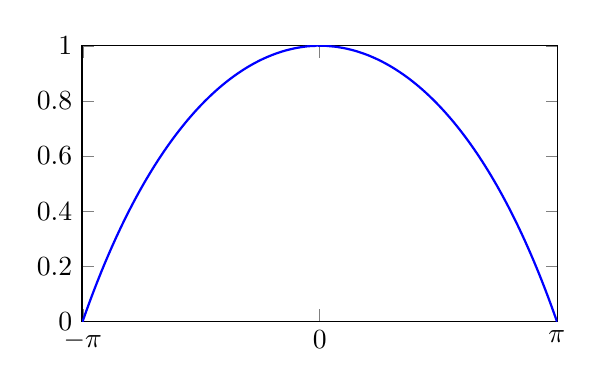
\begin{tikzpicture}
    \begin{axis}
      [
        width=3in,
        height=2in,
        xmin=-3.15,
        xmax=3.15,
        ymin=0,
        ymax=1,
        xtick={-3.14, 0, 3.1415},
        xticklabels={$-\pi$, 0, $\pi$},
      ]
      \addplot[no marks, thick, blue, samples=400]{x/2 * cot(deg(x/2))};
    \end{axis}
  \end{tikzpicture}
  \end{center}
  \caption{Function $x \mapsto \frac{x}{2} \cot \frac{x}{2}$.}
  \label{fig:cot_fcn}
\end{figure}

Let $\epsilon = \lambda_\textrm{max} \left( \textcolor{red}{\left(\mathrm{d}^l \exp_{e_\X} \right)^{-1}} - I \right)$; then we have
\begin{equation}
  \dot V \leq -\begin{bmatrix} \| e_\X \| \\ \| e_v \| \end{bmatrix}^T \begin{bmatrix} c k_p (1 - \epsilon) & -\frac{c k_d}{2} \\ -\frac{c k_d}{2} & k_d - c \end{bmatrix} \begin{bmatrix} \| e_\X \| \\ \| e_v \| \end{bmatrix}
\end{equation}
Therefore, if
\begin{equation}
  \begin{aligned}
    c k_p (1 - \epsilon) + k_d - c \geq 0 \\
    c k_p (1 - \epsilon) - \frac{c^2 k_d^2}{4}  \geq 0
  \end{aligned}
\end{equation}